
\documentclass[12pt,a4paper]{article}

% ------------------------------------------------------------
% Packages
% ------------------------------------------------------------
\usepackage[utf8]{inputenc}
\usepackage[T1]{fontenc}
\usepackage[a4paper,margin=1in]{geometry}
\usepackage{graphicx}
\usepackage{booktabs}
\usepackage{longtable}
\usepackage{array}
\usepackage{float}
\usepackage{caption}
\usepackage{subcaption}
\usepackage{amsmath}
\usepackage{hyperref}
\usepackage{xcolor}
\usepackage{listings}
\usepackage{enumitem}
\usepackage{tikz}
\usepackage{fancyhdr}
\usepackage{lastpage}

\usetikzlibrary{arrows.meta,positioning,shapes.geometric}

% ------------------------------------------------------------
% Hyperref setup
% ------------------------------------------------------------
\hypersetup{
    colorlinks=true,
    linkcolor=blue,
    urlcolor=blue,
    citecolor=blue
}

% ------------------------------------------------------------
% Header and footer
% ------------------------------------------------------------
\pagestyle{fancy}
\fancyhf{}
\lhead{YOLO26n Bowling Score System}
\rhead{Computer Vision Project}
\cfoot{Page \thepage\ of \pageref{LastPage}}

% ------------------------------------------------------------
% Listings setup
% ------------------------------------------------------------
\definecolor{codegray}{rgb}{0.95,0.95,0.95}
\definecolor{codeblue}{rgb}{0.1,0.1,0.55}

\lstset{
    backgroundcolor=\color{codegray},
    basicstyle=\ttfamily\scriptsize,
    breaklines=true,
    frame=single,
    rulecolor=\color{black!30},
    keywordstyle=\color{codeblue}\bfseries,
    commentstyle=\color{green!40!black},
    stringstyle=\color{red!60!black},
    showstringspaces=false,
    tabsize=4,
    columns=fullflexible
}

% ------------------------------------------------------------
% Helper command for figure placeholders
% ------------------------------------------------------------
\newcommand{\placeholderfigure}[2]{
\begin{figure}[H]
    \centering
    \fbox{
        \parbox[c][0.22\textheight][c]{0.82\textwidth}{
            \centering
            \textbf{Figure Placeholder}\\[0.5em]
            #1
        }
    }
    \caption{#2}
\end{figure}
}

% ------------------------------------------------------------
% Title metadata
% ------------------------------------------------------------
\title{\textbf{YOLO26n-Based Bowling Gameplay Analysis and Scoring System}\\
\large End-to-End Model Training, Evaluation, and Video Inference Pipeline}
\author{
Student 1 Name: \underline{\hspace{5cm}} \quad ID: \underline{\hspace{3cm}}\\[0.5em]
Student 2 Name: \underline{\hspace{5cm}} \quad ID: \underline{\hspace{3cm}}
}
\date{\today}

\begin{document}

% ------------------------------------------------------------
% Cover Page
% ------------------------------------------------------------
\begin{titlepage}
    \centering
    \vspace*{1cm}

    \rule{\textwidth}{1pt}\\[0.4cm]
    {\Huge \textbf{YOLO26n-Based Bowling Gameplay Analysis and Scoring System}}\\[0.4cm]
    {\Large \textbf{Model Training, Evaluation, and Bowling Gameplay Inference Report}}\\[0.4cm]
    \rule{\textwidth}{1pt}\\[1.5cm]

\vfill

\begin{center}
\begin{tabular}{c}
\textbf{\large Abdelrahman Abdelrassoul - 202300056} \\[0.45cm]

\textbf{\large Ali Ashraf - 202301812} \\[0.8cm]

\textbf{Submission Date: \today}
\end{tabular}
\end{center}

\vfill
\end{titlepage}

\pagenumbering{roman}
\tableofcontents


\noindent The developed model was later adapted for use in another separate application outside the scope of this report.

\newpage
\listoffigures
\newpage
\listoftables
\newpage
\pagenumbering{arabic}

% ------------------------------------------------------------

\section{Abstract}
% ------------------------------------------------------------

This report documents the complete machine learning and computer vision workflow implemented across two notebooks: \texttt{cv-project-train.ipynb} and \texttt{cv-bonus-test.ipynb}. The project builds a custom YOLO26n object detector for an bowling-bowling scene and evaluates it through both image-level and video-level experiments. The training notebook downloads a Roboflow bowling gameplay dataset, verifies the four target classes, normalizes the bowling gameplay dataset configuration, explores labels, visualizes annotations, trains a YOLO26n detector through transfer learning, evaluates the model on validation and test splits, and runs sample predictions. The testing notebook implements a video-level inference and scoring pipeline that loads trained model files, processes a user-provided video, performs frame-wise detection, tracks pin identities, assigns fall-order labels, draws bowling trajectory paths, saves annotated videos, and writes metrics summaries.

The final trained model achieved strong validation performance with precision of 0.909, recall of 0.880, mAP@0.50 of 0.915, and mAP@0.50:0.95 of 0.744 on the validation split. On the held-out test split, the detector achieved an overall precision of 0.780, recall of 0.745, mAP@0.50 of 0.762, and mAP@0.50:0.95 of 0.444. These results show that the detector learned the task effectively, especially for standing pins, while fallen pins remained more challenging due to occlusion, motion blur, object overlap, and variable orientations. The complete implementation combines lightweight object detection with deterministic temporal tracking to produce a practical video scoring pipeline.

% ------------------------------------------------------------

\section{Introduction}
% ------------------------------------------------------------

The objective of this project is to detect and analyze events in a toy bowling-bowling setup. In this setup, a small remote-controlled bowling collides with bowling pins while a camera records the interaction. The computer vision system must detect objects in the scene, distinguish standing pins from fallen pins, track objects across frames, determine the order in which pins fall, and generate an annotated output video.

The project is divided into two major technical workflows. The first workflow is the model training and evaluation pipeline implemented in \texttt{cv-project-train.ipynb}. This notebook focuses on bowling gameplay dataset loading, validation, preprocessing, YOLO26n transfer learning, evaluation, and prediction visualization. The second workflow is the bowling gameplay inference and scoring pipeline implemented in \texttt{cv-bonus-test.ipynb}. This notebook focuses on applying trained models to full videos rather than still images, maintaining pin identities over time, estimating bowling trajectory, and exporting annotated videos.

This report is written so that the complete implementation can be understood without opening the notebooks. It explains the logic of each major code block, the motivation behind design decisions, the exact metrics extracted from the notebook outputs, and the relationship between detection results and the final scoring logic.

% ------------------------------------------------------------
\section{Problem Statement}
% ------------------------------------------------------------

The problem is a multi-object detection and temporal event analysis task. Given a recorded video of an bowling interacting with bowling pins, the system must identify the relevant objects in each frame and infer higher-level events from frame sequences.

The task is challenging because:
\begin{itemize}[noitemsep]
    \item pins are small and can overlap with each other;
    \item fallen pins can appear in many different orientations;
    \item the bowling moves quickly and can introduce motion blur;
    \item the camera may be handheld, causing frame-to-frame motion;
    \item frame-wise detections alone do not identify which physical pin is which;
    \item duplicate detections may appear on the same object;
    \item a scoring system requires temporal reasoning, not only object detection.
\end{itemize}

Therefore, the final solution requires both a trained object detector and a temporal tracking layer.

% ------------------------------------------------------------

\section{Objectives}
% ------------------------------------------------------------

The project objectives are:
\begin{enumerate}[noitemsep]
    \item collect and use a labeled bowling gameplay dataset for bowling-bowling scenes;
    \item train a lightweight YOLO26n object detector for four classes: ball, bowling, fallen-pins, and standing-pins;
    \item evaluate the detector on validation and test data;
    \item implement a bowling gameplay bowling gameplay analysis pipeline capable of processing complete videos;
    \item track pins across frames using geometric matching;
    \item detect standing-to-fallen transitions and assign fall-order labels;
    \item draw bounding boxes, fall numbers, timing information, and bowling trajectory overlays;
    \item save annotated output videos and model comparison metrics.
\end{enumerate}

% ------------------------------------------------------------
\section{Dataset Description}
% ------------------------------------------------------------

\subsection{Data Source}

The training notebook downloads the bowling gameplay dataset from Roboflow
The exported bowling gameplay dataset is saved under the Kaggle working directory. The bowling gameplay dataset metadata indicates four classes:
\begin{itemize}[noitemsep]
    \item \texttt{ball}
    \item \texttt{bowling}
    \item \texttt{fallen-pins}
    \item \texttt{standing-pins}
\end{itemize}

The notebook verifies these class names explicitly using an assertion. This is important because an incorrect class order would break downstream tracking logic, where class IDs are assumed to map to fixed semantic labels.

\subsection{Dataset Configuration}

The original Roboflow \texttt{data.yaml} initially contains relative paths. The notebook rewrites it to match the Kaggle runtime directory:

\begin{lstlisting}[language=Python]
data_yaml["path"] = DATASET_DIR
data_yaml["train"] = "train/images"
data_yaml["val"] = "valid/images"
data_yaml["test"] = "test/images"
\end{lstlisting}

This ensures that Ultralytics can locate the training, validation, and test folders correctly.

\subsection{Dataset Statistics}

The notebook counts all labels by reading every YOLO label file and accumulating class IDs. Table~\ref{tab:bowling gameplay dataset_stats} summarizes the extracted counts.

\begin{table}[H]
\centering
\caption{Dataset annotation counts extracted from the training notebook.}
\label{tab:bowling gameplay dataset_stats}
\begin{tabular}{lrrrrr}
\toprule
\textbf{Split} & \textbf{ball} & \textbf{bowling} & \textbf{fallen-pins} & \textbf{standing-pins} & \textbf{Total} \\
\midrule
Train & 2323 & 1828 & 8327 & 16681 & 29159 \\
Validation & 210 & 177 & 896 & 1762 & 3045 \\
Test & 112 & 78 & 404 & 742 & 1336 \\
\bottomrule
\end{tabular}
\end{table}

The class distribution is imbalanced. Standing pins dominate the bowling gameplay dataset, followed by fallen pins. The bowling and ball classes are less frequent. This imbalance explains why standing pins achieved the strongest final performance, while ball and fallen-pin detection were comparatively more difficult.

% ------------------------------------------------------------
\section{Data Exploration and Analysis}
% ------------------------------------------------------------

\subsection{File Structure Inspection}

The notebook uses a shell command to inspect the downloaded bowling gameplay dataset:
\begin{lstlisting}[language=bash]
find $DATASET_DIR -maxdepth 3 -type f | head -50
\end{lstlisting}

This verifies that the bowling gameplay dataset contains the expected subdirectories, including image folders and label folders for train, validation, and test splits.

\subsection{Class Name Verification}

The notebook prints and validates the class list:
\begin{lstlisting}[language=Python]
expected_classes = ["ball", "bowling", "fallen-pins", "standing-pins"]
assert data_yaml.get("names") == expected_classes or \
       set(data_yaml.get("names", [])) == set(expected_classes)
\end{lstlisting}

This step prevents mismatched class interpretation during training and inference.

\subsection{Annotation Visualization}

The function \texttt{draw\_yolo\_labels} reads YOLO-format normalized labels, converts them into pixel-space bounding boxes, and draws them over random bowling gameplay frames. This allows visual confirmation that:
\begin{itemize}[noitemsep]
    \item boxes align with the objects;
    \item class IDs correspond to the correct labels;
    \item annotations are suitable for object detection training.
\end{itemize}

% ============================================================
% Dataset Annotation Visualization
% ============================================================

\begin{figure}[H]
\centering

\includegraphics[width=0.9\textwidth]{dataset_annotations.png}
\caption{Dataset annotation visualization for bowling gameplay frames showing bowling ball and pin bounding boxes.}
\label{fig:dataset-annotations}
\end{figure}

% ------------------------------------------------------------
\section{Data Cleaning}
% ------------------------------------------------------------

The bowling gameplay dataset was already exported in YOLO format by Roboflow, but the notebook and Ultralytics training logs performed several cleaning and validation operations:
\begin{itemize}[noitemsep]
    \item missing image-label pairs were avoided by relying on Roboflow's split structure;
    \item duplicate labels were automatically removed by Ultralytics during bowling gameplay dataset scanning;
    \item mixed box/segment information was resolved by using bounding boxes only;
    \item bowling gameplay dataset paths were rewritten in \texttt{data.yaml} for the active runtime.
\end{itemize}

The training output reported multiple duplicate labels removed from several images. This indicates that the training engine detected overlapping or repeated annotation entries and cleaned them before optimization. It also reported that box and segment counts were not equal, so segmentation data were discarded and only detection boxes were used. This is appropriate because the project is an object detection task rather than an instance segmentation task.

% ------------------------------------------------------------
\section{Missing Values Handling}
% ------------------------------------------------------------

The notebooks did not process tabular data, so traditional missing-value imputation was not applicable. Instead, missingness was handled at the bowling gameplay dataset file level:
\begin{itemize}[noitemsep]
    \item the bowling gameplay dataset folder was verified to exist;
    \item image and label folders were checked through directory listing;
    \item labels were read only when corresponding files existed;
    \item Ultralytics bowling gameplay dataset scanning confirmed zero corrupt images in the train, validation, and test splits.
\end{itemize}

The relevant missing-data concept for this project is missing detections during bowling gameplay inference. The testing notebook handles this by giving each pin track a \texttt{missing\_frames} counter and keeping tracks alive for a limited number of frames before removal.

% ------------------------------------------------------------
\section{Feature Engineering}
% ------------------------------------------------------------

For YOLO model training, no handcrafted image features are created. The deep learning model learns hierarchical visual features directly from RGB image data. However, the video-level inference notebook performs geometric feature engineering for tracking and scoring. These derived features include:
\begin{itemize}[noitemsep]
    \item bounding-box center coordinates;
    \item bounding-box area;
    \item IoU between boxes;
    \item Euclidean center distance;
    \item per-track missing-frame count;
    \item fallen-candidate persistence count;
    \item bowling trajectory center points.
\end{itemize}

For a bounding box \(b=(x_1,y_1,x_2,y_2)\), its center is computed as:
\[
c_x = \frac{x_1+x_2}{2}, \qquad c_y = \frac{y_1+y_2}{2}.
\]

The center distance between two boxes \(a\) and \(b\) is:
\[
d(a,b) = \sqrt{(c_{x,a}-c_{x,b})^2 + (c_{y,a}-c_{y,b})^2}.
\]

The IoU between two boxes is:
\[
IoU(A,B)=\frac{|A\cap B|}{|A\cup B|}.
\]

These engineered geometric features allow the system to maintain object identities across frames without training a separate tracker.

% ------------------------------------------------------------
\section{Feature Selection}
% ------------------------------------------------------------

For image detection, feature selection is learned internally by YOLO26n through convolutional and attention-based layers. For tracking, feature selection is rule-based. The test notebook uses only geometry and class identity:
\begin{itemize}[noitemsep]
    \item IoU is selected to preserve spatial overlap continuity;
    \item center distance is selected to handle objects whose boxes move but still represent the same pin;
    \item class ID is selected to determine whether a track should be considered standing or fallen;
    \item confidence is selected to filter weak detections.
\end{itemize}

This design keeps the tracker lightweight and suitable for video analysis.

% ------------------------------------------------------------
\section{Data Preprocessing}
% ------------------------------------------------------------

\subsection{Training Preprocessing}

The training notebook prepares the bowling gameplay dataset by:
\begin{enumerate}[noitemsep]
    \item downloading the Roboflow YOLO26 export;
    \item loading \texttt{data.yaml};
    \item validating class names;
    \item rewriting bowling gameplay dataset paths;
    \item counting labels;
    \item visualizing labels;
    \item feeding the cleaned configuration into Ultralytics.
\end{enumerate}

During training, Ultralytics resizes images to \(640\times640\), batches them, normalizes pixel values internally, applies training augmentations, and converts labels into the format required for YOLO loss computation.

\subsection{Inference Preprocessing}

In the test notebook, each video frame is passed to:
\begin{lstlisting}[language=Python]
model.predict(source=frame, imgsz=640, conf=0.10, iou=0.45)
\end{lstlisting}

Ultralytics handles resizing and normalization internally. Detections are then filtered by class-specific thresholds, converted into NumPy arrays, and passed to the tracking logic.

% ------------------------------------------------------------
\section{Data Augmentation}
% ------------------------------------------------------------

The training command did not manually specify a full custom augmentation block, but the logged Ultralytics trainer configuration shows active default augmentations:
\begin{itemize}[noitemsep]
    \item HSV hue, saturation, and value variation;
    \item translation;
    \item scaling;
    \item horizontal flipping;
    \item mosaic augmentation;
    \item random erasing;
    \item Albumentations blur, median blur, grayscale conversion, and CLAHE.
\end{itemize}

These augmentations are relevant because recorded videos may contain motion blur, lighting variation, camera movement, and object overlap. Mosaic augmentation improves robustness to crowded object layouts, while HSV and blur augmentations improve robustness to appearance variation.

% ------------------------------------------------------------
\section{Data Splitting}
% ------------------------------------------------------------

Roboflow provided train, validation, and test splits. The notebook used:
\begin{itemize}[noitemsep]
    \item \texttt{train/images} for training;
    \item \texttt{valid/images} for validation;
    \item \texttt{test/images} for testing.
\end{itemize}

The validation set was used during training to monitor generalization and trigger early stopping. The test set was used after training to estimate final held-out performance.

% ------------------------------------------------------------
\section{Model Architecture}
% ------------------------------------------------------------

\subsection{YOLO26n Overview}

The model used in the training notebook is:
\begin{lstlisting}[language=Python]
model = YOLO("yolo26n.pt")
\end{lstlisting}

YOLO26n is a compact single-stage detector. It predicts bounding boxes and class probabilities directly from image features. The training log reports:
\begin{itemize}[noitemsep]
    \item 260 layers before fusion;
    \item 2,505,360 parameters during training;
    \item 5.8 GFLOPs;
    \item 4 output classes.
\end{itemize}

After fusion for validation, the model summary reports:
\begin{itemize}[noitemsep]
    \item 122 layers;
    \item 2,375,616 parameters;
    \item 5.2 GFLOPs.
\end{itemize}

\subsection{Architecture Blocks}

The printed architecture includes:
\begin{itemize}[noitemsep]
    \item convolutional downsampling layers;
    \item C3k2 feature extraction blocks;
    \item SPPF spatial pyramid pooling;
    \item C2PSA attention-style processing;
    \item upsampling and concatenation layers for feature fusion;
    \item a Detect head with feature maps from three scales.
\end{itemize}

The three-scale detection head is important because pins and the bowling can appear at different sizes depending on camera distance.

\subsection{Input and Output Shapes}

The exported PyTorch model uses input shape:
\[
(1,3,640,640),
\]
where the dimensions represent batch size, RGB channels, height, and width. The exported TensorFlow model reports output shape:
\[
(1,300,6),
\]
which corresponds to up to 300 detections, each containing:
\[
[x_1, y_1, x_2, y_2, confidence, class\_id].
\]

% ------------------------------------------------------------
\section{Model Design Decisions}
% ------------------------------------------------------------

YOLO26n was selected because the task benefits from a compact detector that can process many video frames efficiently. A larger detector may improve accuracy but would increase latency and memory usage. A nano-scale model provides a practical trade-off between detection quality and computational cost.

Transfer learning was used instead of training from scratch. The log reports that 606 out of 708 pretrained items were transferred. This is beneficial because early convolutional filters already encode general visual patterns such as efficients, corners, textures, and local shapes. Fine-tuning adapts those representations to the specific bowling-bowling classes.

The detector is intentionally paired with a rule-based temporal tracker rather than a heavy neural video model. This keeps the video analysis pipeline simpler and computationally efficient.

% ------------------------------------------------------------
\section{Training Pipeline}
% ------------------------------------------------------------

The training call is:
\begin{lstlisting}[language=Python]
model.train(
    data=data_yaml_path,
    epochs=100,
    imgsz=640,
    batch=16,
    device=0,
    workers=2,
    pretrained=True,
    optimizer="AdamW",
    lr0=0.001,
    lrf=0.01,
    weight_decay=0.0005,
    patience=25,
    cos_lr=True,
    project="/kaggle/working/runs",
    name="rc_bowling_yolo26n_no_extra_aug",
    exist_ok=True
)
\end{lstlisting}

The training was performed on a Tesla T4 GPU. Automatic Mixed Precision checks passed, allowing faster training and lower GPU memory usage.

\subsection{Hyperparameters}

\begin{table}[H]
\centering
\caption{Main training hyperparameters used in the notebook.}
\label{tab:hyperparameters}
\begin{tabular}{ll}
\toprule
\textbf{Hyperparameter} & \textbf{Value} \\
\midrule
Model & YOLO26n \\
Epochs & 100 maximum \\
Completed epochs & 96 due to early stopping \\
Best epoch & 71 \\
Image size & 640 \\
Batch size & 16 \\
Optimizer & AdamW \\
Initial learning rate & 0.001 \\
Final LR factor & 0.01 \\
Weight decay & 0.0005 \\
Patience & 25 \\
Scheduler & Cosine LR \\
Workers & 2 \\
Device & Tesla T4 GPU \\
Framework & Ultralytics 8.4.46 / PyTorch 2.10.0 \\
\bottomrule
\end{tabular}
\end{table}

% ------------------------------------------------------------
\section{Loss Functions}
% ------------------------------------------------------------

The YOLO training log reports three loss components:
\begin{itemize}[noitemsep]
    \item \textbf{Box loss:} localization error between predicted and ground-truth boxes;
    \item \textbf{Class loss:} classification error for object classes;
    \item \textbf{DFL loss:} distribution focal loss used for bounding-box regression precision.
\end{itemize}

The overall optimization objective can be described as:
\[
\mathcal{L}_{total} =
\lambda_{box}\mathcal{L}_{box}
+
\lambda_{cls}\mathcal{L}_{cls}
+
\lambda_{dfl}\mathcal{L}_{dfl}.
\]

During backpropagation, gradients of this total loss update model parameters through AdamW.

% ------------------------------------------------------------
\section{Optimizer and Learning Rate Strategy}
% ------------------------------------------------------------

AdamW was used as the optimizer:
\[
\theta_{t+1} = \theta_t - \eta \cdot \hat{m}_t / (\sqrt{\hat{v}_t}+\epsilon) - \eta\lambda\theta_t,
\]
where the last term represents decoupled weight decay. This optimizer is suitable for deep learning models because it combines adaptive gradient moments with explicit regularization.

Cosine learning-rate scheduling was enabled. This gradually decays the learning rate from the initial value toward the final factor, allowing large updates early and more stable refinement later.

% ------------------------------------------------------------
\section{Training Procedure}
% ------------------------------------------------------------

Training progressed for 96 epochs and stopped early because no improvement was observed for 25 epochs. The best checkpoint was saved at epoch 71. The early stopping behavior prevented unnecessary overfitting and reduced wasted computation.

The model improved rapidly in the first ten epochs:
\begin{itemize}[noitemsep]
    \item mAP@0.50 increased from 0.590 at epoch 1 to 0.872 at epoch 10;
    \item mAP@0.50:0.95 increased from 0.407 to 0.671 over the same interval.
\end{itemize}

Performance then stabilized gradually, with the best validation result observed around epoch 71.

% ============================================================
% Training Loss Curves
% ============================================================

\begin{figure}[H]
\centering

\includegraphics[width=0.9\textwidth]{Train-loss.png}
\caption{Training and validation loss curves over epochs for the bowling gameplay analysis model.}
\label{fig:training-loss-curves}
\end{figure}

% ============================================================
% Validation Precision, Recall, and F1
% ============================================================

\begin{figure}[H]
\centering

\includegraphics[width=0.9\textwidth]{val-per-rec-f1.png}
\caption{Validation precision, recall, and F1-related performance trends across training epochs.}
\label{fig:validation-metrics}
\end{figure}

% ============================================================
% Validation mAP Curves
% ============================================================

\begin{figure}[H]
\centering

\includegraphics[width=0.9\textwidth]{val-mAP.png}
\caption{Validation mAP@0.50 and mAP@0.50:0.95 curves for bowling ball and pin detection.}
\label{fig:validation-map-curves}
\end{figure}

% ============================================================
% Confusion Matrix
% ============================================================

\begin{figure}[H]
\centering

\includegraphics[width=0.85\textwidth]{confusion_matrix_normalized.png}
\caption{Normalized Confusion matrix for bowling gameplay object detection and pin-state classification.}
\label{fig:confusion-matrix}
\end{figure}

% ============================================================
% Precision-Recall Curve
% ============================================================

\begin{figure}[H]
\centering

\includegraphics[width=0.85\textwidth]{BoxPR_curve.png}
\caption{Precision--recall curve for bowling ball and pin detection performance.}
\label{fig:precision-recall-curve}
\end{figure}

% ============================================================
% F1-Confidence Curve
% ============================================================

\begin{figure}[H]
\centering

\includegraphics[width=0.85\textwidth]{BoxF1_curve.png}
\caption{F1-confidence curve showing the effect of confidence threshold selection on bowling gameplay detection performance.}
\label{fig:f1-confidence-curve}
\end{figure}

% ============================================================
% Precision-Confidence Curve
% ============================================================

\begin{figure}[H]
\centering

\includegraphics[width=0.85\textwidth]{BoxP_curve.png}
\caption{Precision-confidence curve showing precision variation across confidence thresholds for bowling gameplay detection.}
\label{fig:precision-confidence-curve}
\end{figure}

% ============================================================
% Recall-Confidence Curve
% ============================================================

\begin{figure}[H]
\centering

\includegraphics[width=0.85\textwidth]{BoxR_curve.png}
\caption{Recall-confidence curve showing recall variation across confidence thresholds for bowling gameplay detection.}
\label{fig:recall-confidence-curve}
\end{figure}

% ------------------------------------------------------------
\section{Validation Logic}
% ------------------------------------------------------------

Validation was performed automatically after every epoch during training. The notebook also explicitly called:
\begin{lstlisting}[language=Python]
metrics = model.val(
    data=data_yaml_path,
    split="val",
    imgsz=640,
    conf=0.25,
    iou=0.5,
    device=0
)
\end{lstlisting}

This evaluates predictions against ground-truth boxes using a confidence threshold of 0.25 and IoU threshold of 0.5.

% ------------------------------------------------------------
\section{Evaluation Metrics}
% ------------------------------------------------------------

The notebooks report object detection metrics:
\begin{itemize}[noitemsep]
    \item Precision;
    \item Recall;
    \item mAP@0.50;
    \item mAP@0.50:0.95;
    \item inference speed;
    \item per-class detection results.
\end{itemize}

Precision and recall are defined as:
\[
Precision=\frac{TP}{TP+FP},
\qquad
Recall=\frac{TP}{TP+FN}.
\]

The F1-score is computed as:
\[
F1 = 2\cdot\frac{Precision\cdot Recall}{Precision+Recall}.
\]

The notebooks did not log classification accuracy or ROC/AUC because YOLO object detection is evaluated primarily through localization-sensitive detection metrics rather than image-level classification metrics. Confusion matrix and curve plots are generated by Ultralytics when \texttt{plots=True}, but their numeric matrices are not explicitly printed in the notebook.

% ------------------------------------------------------------
\section{Experimental Results}
% ------------------------------------------------------------

\subsection{Final Validation Results}

\begin{table}[H]
\centering
\caption{Final validation metrics for the best YOLO26n checkpoint.}
\label{tab:val_metrics}
\begin{tabular}{lrrrrrr}
\toprule
\textbf{Class} & \textbf{Images} & \textbf{Instances} & \textbf{Precision} & \textbf{Recall} & \textbf{mAP50} & \textbf{mAP50-95} \\
\midrule
all & 240 & 2983 & 0.909 & 0.880 & 0.915 & 0.744 \\
ball & 129 & 203 & 0.853 & 0.872 & 0.886 & 0.637 \\
bowling & 167 & 174 & 0.961 & 0.853 & 0.915 & 0.707 \\
fallen-pins & 210 & 890 & 0.867 & 0.835 & 0.894 & 0.749 \\
standing-pins & 230 & 1716 & 0.957 & 0.961 & 0.963 & 0.882 \\
\bottomrule
\end{tabular}
\end{table}

Standing pins achieved the highest mAP@0.50 because they are visually more consistent and more frequent in the training set. Fallen pins were harder because their appearance changes significantly after impact.

\subsection{Held-Out Test Results}

\begin{table}[H]
\centering
\caption{Held-out test metrics reported by the notebook.}
\label{tab:test_metrics}
\begin{tabular}{lrrrrrr}
\toprule
\textbf{Class} & \textbf{Images} & \textbf{Instances} & \textbf{Precision} & \textbf{Recall} & \textbf{mAP50} & \textbf{mAP50-95} \\
\midrule
all & 120 & 1336 & 0.780 & 0.745 & 0.762 & 0.444 \\
ball & 63 & 112 & 0.701 & 0.705 & 0.686 & 0.320 \\
bowling & 77 & 78 & 0.681 & 0.821 & 0.807 & 0.418 \\
fallen-pins & 104 & 404 & 0.788 & 0.653 & 0.674 & 0.431 \\
standing-pins & 114 & 742 & 0.952 & 0.800 & 0.879 & 0.606 \\
\bottomrule
\end{tabular}
\end{table}

The test results are lower than validation results, showing a realistic generalization gap. The largest difficulty occurs for fallen pins and balls, likely because they appear in more variable positions and can be partially occluded.

\subsection{Inference Speed}

The best validation run reported:
\begin{table}[H]
\centering
\caption{Validation speed reported by Ultralytics.}
\begin{tabular}{lr}
\toprule
\textbf{Stage} & \textbf{Time per image} \\
\midrule
Preprocessing & 0.2 ms \\
Inference & 2.2 ms \\
Loss & 0.0 ms \\
Postprocessing & 2.3 ms \\
\bottomrule
\end{tabular}
\end{table}

The explicit held-out test run reported 1.9 ms preprocessing, 6.6 ms inference, and 2.6 ms postprocessing per image.

% ------------------------------------------------------------
\section{Testing Pipeline}
% ------------------------------------------------------------

The training notebook performs image-level prediction on the test set:
\begin{lstlisting}[language=Python]
model.predict(
    source=TEST_IMAGE_DIR,
    imgsz=640,
    conf=0.20,
    iou=0.45,
    save=True,
    project="/kaggle/working/predictions",
    name="test_predictions",
    exist_ok=True
)
\end{lstlisting}

This saves annotated prediction images for visual inspection. The output logs show detections for each test image, including the number of balls, fallen pins, and standing pins detected.

% ============================================================
% Test Prediction Results
% ============================================================

\begin{figure}[H]
\centering

\includegraphics[width=0.9\textwidth]{pred-labels.png}
\caption{YOLO26n prediction results on bowling gameplay frames showing detected bowling balls and pins.}
\label{fig:test-prediction-results}
\end{figure}

% ------------------------------------------------------------

\section{Model Checkpoint Selection and Benchmarking}
% ------------------------------------------------------------

After training, the best checkpoint was selected automatically using the validation performance tracked by Ultralytics. Early stopping identified epoch 71 as the best epoch, and the corresponding weights were saved as \texttt{best.pt}. This checkpoint was then used for image-level test prediction and for the video-level scoring pipeline.

\subsection{Benchmark Results}

The notebook also reported benchmark measurements for selected runtime formats. These measurements are useful for understanding the computational cost of the detector under the notebook runtime conditions.

\begin{table}[H]
\centering
\caption{Selected model benchmark results reported by the notebook.}
\begin{tabular}{lrrrr}
\toprule
\textbf{Format} & \textbf{Status} & \textbf{Size (MB)} & \textbf{mAP50-95} & \textbf{FPS} \\
\midrule
PyTorch & Success & 19.8 & 0.6013 & 80.75 \\
TensorRT & Success & 11.4 & 0.6004 & 314.40 \\
TensorFlow SavedModel & Success & 23.5 & 0.6004 & 49.37 \\
\bottomrule
\end{tabular}
\end{table}

The benchmark results show that the trained detector is computationally lightweight. The main experimental checkpoint remains the PyTorch \texttt{best.pt} model used throughout the reported bowling gameplay inference experiments.

% ------------------------------------------------------------
\section{Video Inference Pipeline}
% ------------------------------------------------------------

The notebook \texttt{cv-bonus-test.ipynb} implements the full video scoring pipeline. It begins by installing dependencies, importing libraries, finding available videos and models, setting a single input video path, and creating an output directory.


\subsection{Model Loading}

The video testing notebook sets explicit paths for the trained model and input video. The primary model is loaded through the Ultralytics \texttt{YOLO(model\_path)} interface. This design allows the same video processing function to be applied to a selected checkpoint while keeping the inference and tracking logic independent from the training code.

\subsection{Video Processor}

The core function \texttt{run\_video\_scoring}:
\begin{enumerate}[noitemsep]
    \item loads one model using \texttt{YOLO(model\_path)};
    \item opens the input video with OpenCV;
    \item obtains FPS, width, height, and frame count;
    \item creates an MP4 writer;
    \item processes frames sequentially;
    \item runs YOLO prediction per frame;
    \item filters detections by confidence and class;
    \item updates pin tracks;
    \item draws annotations;
    \item saves frame-level logs;
    \item writes summary JSON and metrics CSV.
\end{enumerate}

\subsection{Video Data Flow Diagram}

\begin{figure}[H]
\centering
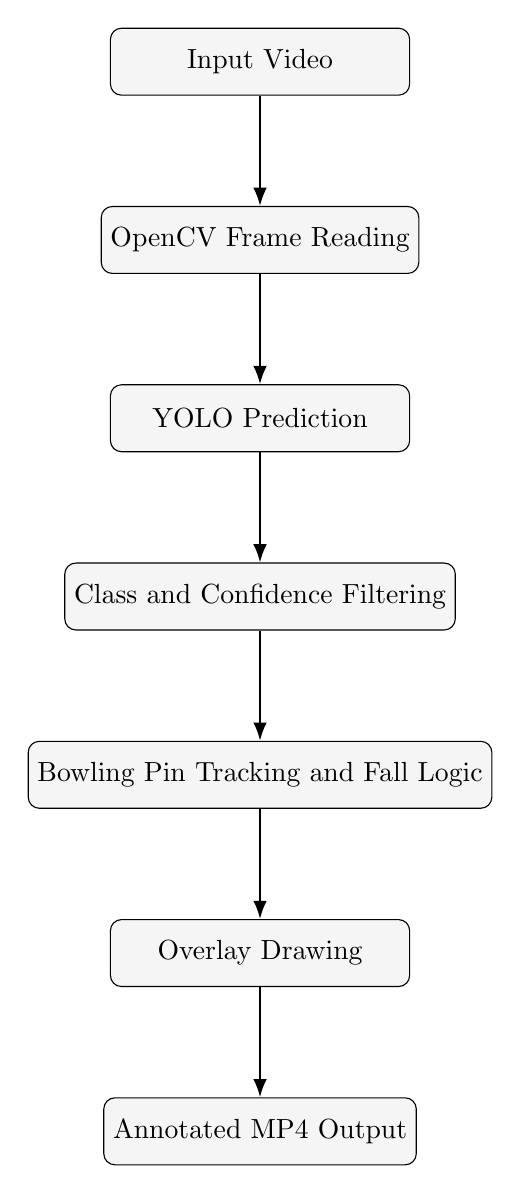
\begin{tikzpicture}[
    node distance=1.4cm,
    block/.style={draw, rounded corners, align=center, minimum width=3.8cm, minimum height=0.85cm, fill=gray!8},
    arrow/.style={-Latex, thick}
]
\node[block] (video) {Input Video};
\node[block, below=of video] (frame) {OpenCV Frame Reading};
\node[block, below=of frame] (detect) {YOLO Prediction};
\node[block, below=of detect] (filter) {Class and Confidence Filtering};
\node[block, below=of filter] (track) {Bowling Pin Tracking and Fall Logic};
\node[block, below=of track] (overlay) {Overlay Drawing};
\node[block, below=of overlay] (write) {Annotated MP4 Output};

\draw[arrow] (video) -- (frame);
\draw[arrow] (frame) -- (detect);
\draw[arrow] (detect) -- (filter);
\draw[arrow] (filter) -- (track);
\draw[arrow] (track) -- (overlay);
\draw[arrow] (overlay) -- (write);
\end{tikzpicture}
\caption{Video inference and scoring pipeline implemented in the testing notebook.}
\end{figure}

% ------------------------------------------------------------
\section{Prediction Logic}
% ------------------------------------------------------------

For each processed frame, the notebook executes:
\begin{lstlisting}[language=Python]
results = model.predict(
    source=frame,
    imgsz=640,
    conf=0.10,
    iou=0.45,
    verbose=False
)[0]
\end{lstlisting}

Each box is converted into:
\begin{itemize}[noitemsep]
    \item class ID;
    \item confidence score;
    \item \((x_1,y_1,x_2,y_2)\) bounding box.
\end{itemize}

The code then applies per-class confidence thresholds:
\begin{table}[H]
\centering
\caption{Class-specific thresholds in the video testing notebook.}
\begin{tabular}{lr}
\toprule
\textbf{Class} & \textbf{Threshold} \\
\midrule
ball & 0.15 \\
bowling & 0.15 \\
fallen-pins & 0.12 \\
standing-pins & 0.12 \\
\bottomrule
\end{tabular}
\end{table}

The lower thresholds improve recall in video frames, where motion blur may reduce confidence. However, they can also increase false positives and duplicate detections, which is why tracking and duplicate-control logic are important.

% ------------------------------------------------------------
\section{Tracking Logic}
% ------------------------------------------------------------

\subsection{PinTrack Class}

The testing notebook defines a \texttt{PinTrack} class. Each track stores:
\begin{itemize}[noitemsep]
    \item track ID;
    \item latest bounding box;
    \item last seen frame;
    \item missing-frame count;
    \item current state;
    \item last class ID;
    \item confidence score;
    \item fallen-candidate count;
    \item fall order;
    \item fall frame;
    \item history.
\end{itemize}

This class transforms independent detections into persistent temporal objects.

\subsection{Matching Strategy}

For each existing track, the algorithm searches the current pin detections and computes:
\[
score = 2\cdot IoU - \frac{distance}{CENTER\_DISTANCE\_THRESHOLD}.
\]

A detection can match a track if:
\[
IoU \geq 0.10
\quad \text{or} \quad
distance \leq 160.
\]

The best scoring match updates the track. If no detection matches, the track is marked missing.

\subsection{Track Creation and Removal}

Unmatched pin detections create new tracks if their confidence is at least 0.12. Tracks are removed if missing for more than 25 frames. This design allows temporary missed detections while preventing old tracks from remaining forever.

\subsection{Fall Confirmation}

A track becomes confirmed as fallen when its \texttt{fallen\_candidate\_count} reaches 3. This means the same tracked pin must be classified as fallen across multiple updates before a fall order is assigned. This temporal requirement reduces false scoring from single-frame misclassification.

% ------------------------------------------------------------
\section{Overlay Rendering}
% ------------------------------------------------------------

The testing notebook uses OpenCV drawing functions to render:
\begin{itemize}[noitemsep]
    \item yellow ball boxes;
    \item magenta bowling boxes and trajectory;
    \item green active standing pin tracks;
    \item red confirmed fallen pin tracks;
    \item numbered circles for fall order;
    \item top-left summary panel containing model name, elapsed time, and fallen count.
\end{itemize}

The output video is written frame by frame through \texttt{cv2.VideoWriter} using MP4 encoding.

% ------------------------------------------------------------
\section{Metrics and Output Files from Video Testing}
% ------------------------------------------------------------

For every tested model, the video notebook saves:
\begin{itemize}[noitemsep]
    \item annotated video;
    \item frame-level CSV metrics;
    \item summary JSON file;
    \item final comparison CSV.
\end{itemize}

The summary includes:
\begin{itemize}[noitemsep]
    \item model name and path;
    \item input video path;
    \item output path;
    \item FPS;
    \item width and height;
    \item total frames;
    \item processing runtime;
    \item processing FPS;
    \item final fallen count;
    \item total active tracks;
    \item number of bowling-path points.
\end{itemize}

% ------------------------------------------------------------
\section{Error Analysis}
% ------------------------------------------------------------

The implementation and notebook outputs reveal several important error sources:
\begin{itemize}
    \item \textbf{Fallen-pin ambiguity:} fallen pins appear in many orientations, leading to lower recall and mAP than standing pins.
    \item \textbf{Duplicate detections:} the test prediction logs show images with many predicted standing pins, which may exceed the number of physical pins in the scene.
    \item \textbf{Class imbalance:} standing pins dominate the bowling gameplay dataset, improving their performance but making minority classes more challenging.
    \item \textbf{Video motion blur:} fast bowling motion and falling pins can reduce detector confidence.
    \item \textbf{Generalization gap:} validation mAP@0.50:0.95 was 0.744, while held-out test mAP@0.50:0.95 was 0.444.
\end{itemize}

The video notebook addresses some errors through temporal tracking and fall confirmation, but detection quality remains the foundation of the scoring system.

% ------------------------------------------------------------

\section{Performance Analysis}
% ------------------------------------------------------------

The YOLO26n detector provides strong speed because it is small and computationally efficient. Validation inference speed was approximately 2.2 ms per image in the best validation run. The benchmark cell reported PyTorch inference at 12.38 ms per image and approximately 80.75 FPS under its benchmark conditions. TensorRT achieved 3.18 ms per image and 314.4 FPS in the notebook benchmark.

The video pipeline adds additional cost beyond single-image inference because it performs frame decoding, detection filtering, geometric matching, overlay drawing, output writing, and metrics logging. Therefore, complete video runtime is determined by both detector speed and the surrounding frame-processing operations.

% ------------------------------------------------------------

\section{Challenges Faced}
% ------------------------------------------------------------

The main challenges were:
\begin{itemize}
    \item \textbf{Small-object detection:} pins and balls occupy small image regions.
    \item \textbf{State classification:} fallen and standing pins are visually related but semantically different.
    \item \textbf{Temporal identity:} YOLO detections do not automatically preserve object identity across frames.
    \item \textbf{Duplicate detections:} low inference thresholds improve recall but increase false positives.
    \item \textbf{Video ambiguity:} camera movement, fast bowling motion, and pin overlap introduce frame-level instability.
\end{itemize}

% ------------------------------------------------------------

\section{Future Improvements}
% ------------------------------------------------------------

Future improvements include:
\begin{itemize}[noitemsep]
    \item collecting more test-like videos with varied lighting, camera angles, and pin layouts;
    \item cleaning duplicate annotations before training;
    \item adding explicit duplicate suppression in the bowling gameplay inference notebook;
    \item using stronger temporal fall confirmation rules;
    \item locking the initial pin count to prevent fake mid-video tracks;
    \item integrating ByteTrack or BoT-SORT more consistently into the custom scoring layer;
    \item expanding evaluation with more annotated video-level ground truth.
\end{itemize}

% ------------------------------------------------------------

\section{Conclusion}
% ------------------------------------------------------------

The two notebooks implement a complete object detection and video scoring pipeline for bowling-bowling analysis. The training notebook successfully prepares a Roboflow bowling gameplay dataset, trains a YOLO26n detector, evaluates it, and visualizes predictions. The testing notebook applies trained models to complete videos, tracks pins through time, confirms fall events, draws annotations, and exports result videos with frame-level metrics.

The final detector achieved strong validation performance, especially on standing pins, and the video pipeline demonstrates how frame-level detections can be converted into higher-level scoring events through deterministic temporal logic. The project therefore combines deep learning detection with classical geometric tracking to solve a practical video understanding and scoring problem.



\bibitem{ultralytics}
Ultralytics, \textit{YOLO Documentation and Training Framework}. Available: \url{https://docs.ultralytics.com/}

\bibitem{roboflow}
Roboflow, \textit{Dataset Management and Annotation Platform}. Available: \url{https://roboflow.com/}

\bibitem{opencv}
OpenCV, \textit{Open Source Computer Vision Library}. Available: \url{https://opencv.org/}

\end{document}
